As a testcase to learn how to use the PLUTO software we simulated hydrodynamic and magnetohydrodynamicblastwaves in a 2D domain. The initial condition for the simulations is a circle with radius $0.3$ (in code units) with higher pressure.
The pressure outside the circle is $1$, in code units. For the pressure inside the circle two scenarios were simulated.
One with a large pressure difference, where the pressure inside the circle is $5$. In the other scenario a lower pressure difference was used: the pressure inside the circle was $1.5$
The reason for using different pressure differences is to see the non-linear effects in the shock-wave with high pressure difference.

\subsection{Hydrodynamic blastwave}
In \autoref{fig:HD-blast-short} the pressureprofile of both scenarios is plot for the initial condition and two frames right after the start of the simulation.
In \autoref{fig:HD-blast-long} the profile is plotted for later times.

\begin{figure}[h]
	%\hspace{-1cm}
	\centering
	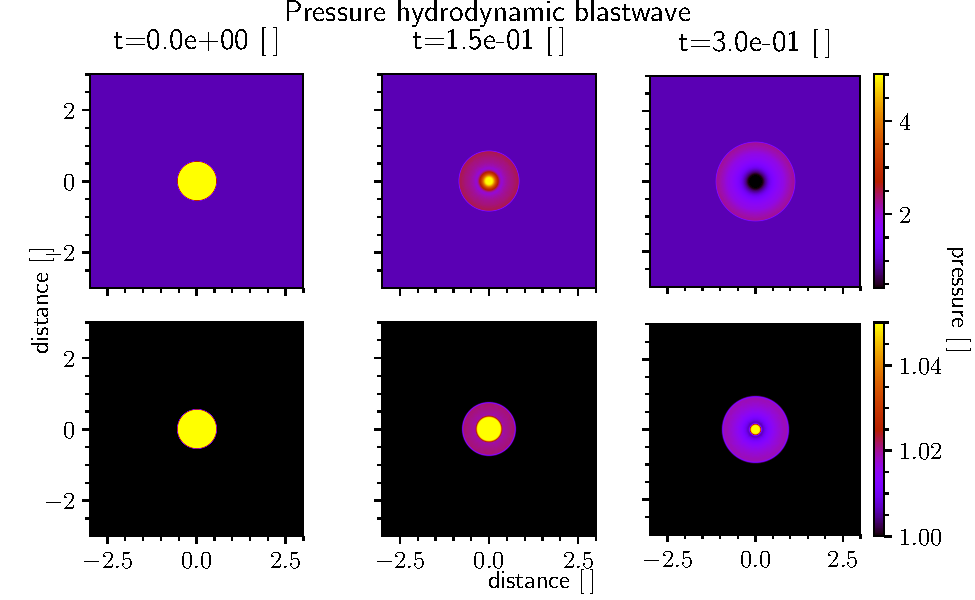
\includegraphics[width=\linewidth]{images/HD-blast-prs-1.pdf}
	\caption{Pressure profile for a blastwave in an ideal fluid at different times. The top row start with the larger pressure difference of $5/1$, the bottom row is the blastwave with smaller pressure difference of $1.5/1$.}
	\label{fig:HD-blast-short}
\end{figure}

\begin{figure}[h]
	%\hspace{-1cm}
	\centering
	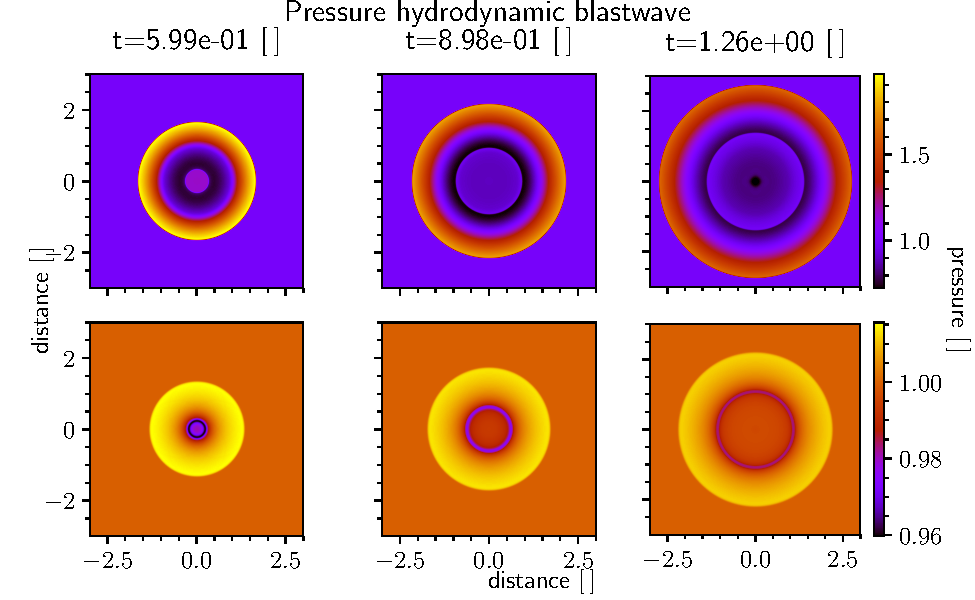
\includegraphics[width=\linewidth]{images/HD-blast-prs-2.pdf}
	\caption{Pressure profile for a blastwave in an ideal fluid at larger timescales. Initial conditions for each row are the same as in \autoref{fig:HD-blast-short}.}
	\label{fig:HD-blast-long}
\end{figure}

test
